\bartchapterimage{potw1252a.jpg}
\chapter{Conclusions and perspectives}
\label{cha:conclusions_and_perspectives}
\bartthumb{potw1252a.png}

\section{Conclusions}
\label{sec:conclusions}

The optimal extraction of galaxy groups from redshift space is not an easy
task. The observer has to deal with observational errors, projection
effects and bias to perform such an optimal grouping. We have argued that all
previously created galaxy group algorithms are imperfect in the sense that with
their assumptions, there are some lacks in extracted groups, explaining the
apparition of two different kind of algorithms: Bayesian and geometrical.

We constructed a galaxy mock catalogue to test several grouping algorithms. We
tested Friends-of-Friends algorithm to understand what is the optimal set of
linking lengths. We conclude that the choice of optimal linking lengths depends
on the science one wishes to do.

We created  MAGGIE, a Bayesian galaxy group finder, using probabilities to
constrain the membership in groups. The virial radii are estimated from either
the stellar mass (MAGGIE-m) or the luminosity (MAGGIE-L) of the central galaxy.
We show by tests on our mock catalogues that both implementations of MAGGIE
perform better on perfect data with no observational errors than the optimal
FoF algorithm. We also show that Bayesian algorithms as MAGGIE are more
sensitive to the quality of observational data than geometrical ones as FoF.
Nevertheless, both MAGGIE-m (with 0.02 dex errors in stellar masses) and
MAGGIE-L (with 0.08 dex errors in observed luminosities) perform better than
the optimal FoF, except at very high group masses, where the abundance matching
technique used in MAGGIE becomes inaccurate.

The application of MAGGIE on real galaxy surveys implies a full understanding
of the possible incompletenesses of these surveys. The analysis of the
SDSS-DR10 indicates that correcting for luminous and spectroscopic
incompletenesses is very important but also very difficult, since the
extraction of galaxy groups implies no missing galaxies. Incomplete membership
can affect the grouping, but also the informations obtained from their
analysis. Indeed, environmental effects we wish to observe in galaxy groups
(essentially through the SSFR) can be very sensitive to the way incompleteness
is handled. Therefore, MAGGIE is a very powerful tool for galaxy group analysis, but we have
to apply it carefully on the analysed data or the interpretation of results can
be biased.

\section{Perspectives}
\label{sec:perspectives}

We plan to run MAGGIE on the SDSS-DR10 and publish optimized galaxy groups in
different doubly complete subsamples in redshift and luminosity, and to
re-assess the modulation of sSFR, etc\ldots with local and global environments.
If a modulation of galaxy properties is observed, we will model it and apply it
in semi-analytical codes to see if it reduces discrepancies between
observations and outputs of such codes. It will be a new measure of quenching
of star formation with global and local environments. We also wish to run
MAGGIE on the deeper GAMA redshift survey to be able to extract the evolution
in time of environmental effects on galaxies. We already have some preliminary
results on this modulation applying MAGGIE on the SDSS\@.
\bartreffigure{ssfr_mean} and \bartreffigure{ssfr_fraction} show the median
SSFR and the fraction of non-passive galaxies with local and global environment
for the SDSS, and the same for group catalogues of~\cite{Tempel+14} in
\bartreffigure{ssfr_mean_tempel} and \bartreffigure{ssfr_fraction_tempel}. We
use two complete catalogues to show this modulation: catalogue 3 too have
sufficient statistics in number of galaxies and catalogue 5 to see the
behaviour at larger redshifts.

\begin{figure}[htb]
    \centering
    \begin{minipage}{\linewidth}
        \centering
        \begin{minipage}{\linewidth}
            \centering
            \subfloat[Catalogue 3]{%
                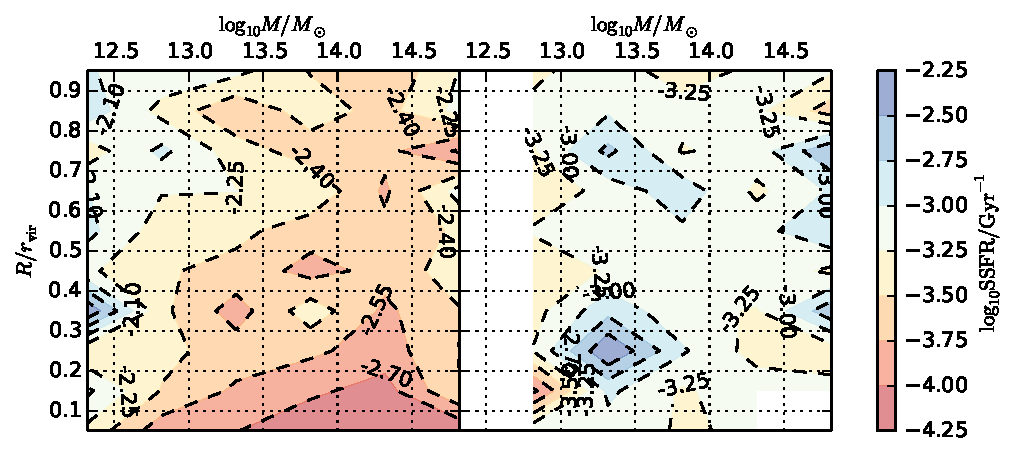
\includegraphics[height=0.2\textheight]{%
                    {figures/maggie_vs_sdss/sdss.0.mean_ssfr_2}.pdf%
                }
            }
        \end{minipage}
        \begin{minipage}{\linewidth}
            \centering
            \subfloat[Catalogue 5]{%
                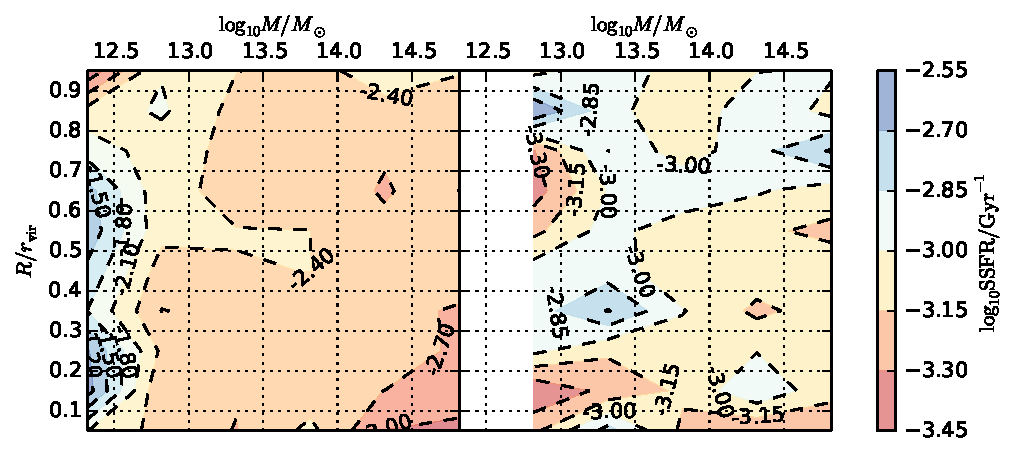
\includegraphics[height=0.2\textheight]{%
                    {figures/maggie_vs_sdss/sdss.0.mean_ssfr_4}.pdf%
                }
            }
        \end{minipage}
        \captionof{figure}{Mean SSFR for galaxies with
            $10\leqslant\log_{10}m_*<11$ (left panel) and
            $11\leqslant\log_{10}m_*<12$ in function of the projected radius
            in units of virial radius (local environment) and of the virial
            mass in solar units (global environment), for galaxy groups
        found with MAGGIE.\label{fig:ssfr_mean}}
    \end{minipage}
    \begin{minipage}{\linewidth}
        \centering
        \begin{minipage}{\linewidth}
            \centering
            \subfloat[Catalogue 3]{%
                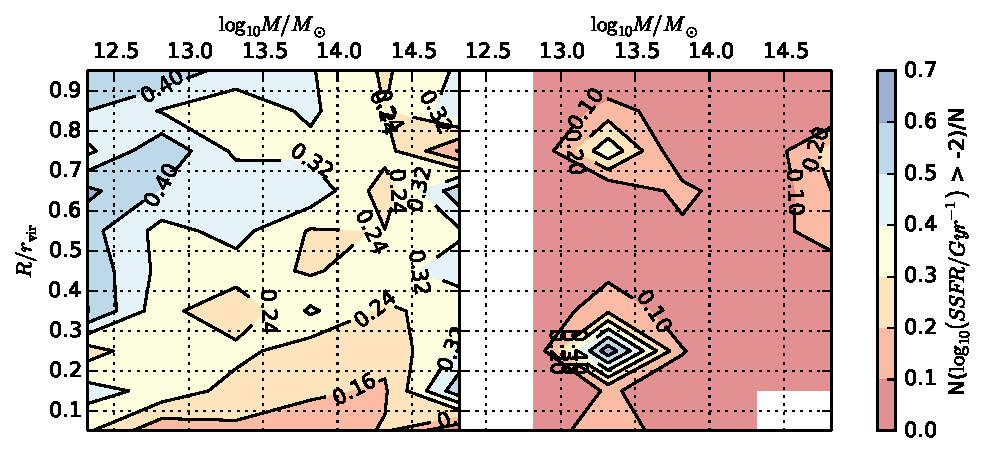
\includegraphics[height=0.2\textheight]{%
                    {figures/maggie_vs_sdss/sdss.0.fraction_over_minus_2_2}.pdf%
                }
            }
        \end{minipage}
        \begin{minipage}{\linewidth}
            \centering
            \subfloat[Catalogue 5]{%
                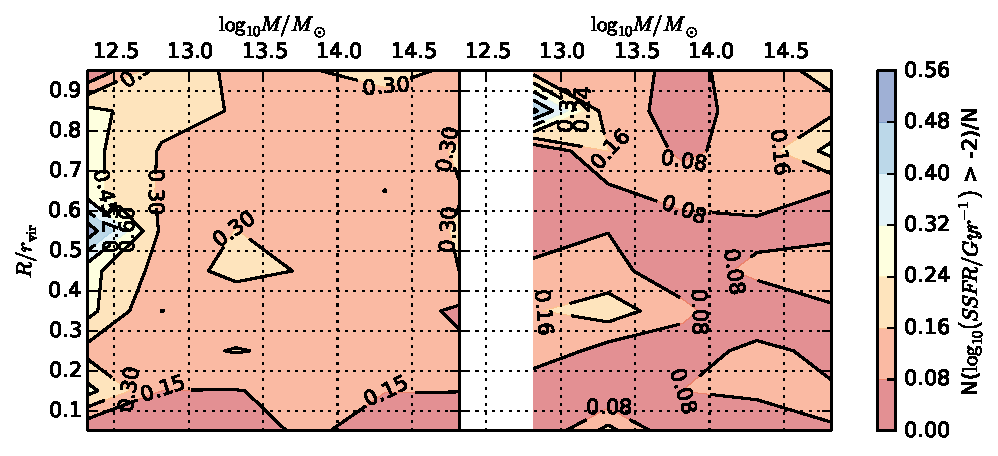
\includegraphics[height=0.2\textheight]{%
                    {figures/maggie_vs_sdss/sdss.0.fraction_over_minus_2_4}.pdf%
                }
            }
        \end{minipage}
        \captionof{figure}{Fraction of galaxies classified as star forming
            galaxies according the criterion of
            \bartrefsubsection{star_formation_rate} for the same range in
            stellar masses as in \bartreffigure{ssfr_mean}, with galaxy group
            from MAGGIE.\label{fig:ssfr_fraction}}
    \end{minipage}
\end{figure}

\begin{figure}[htb]
    \centering
    \begin{minipage}{\linewidth}
        \centering
        \begin{minipage}{\linewidth}
            \centering
            \subfloat[Catalogue 3]{%
                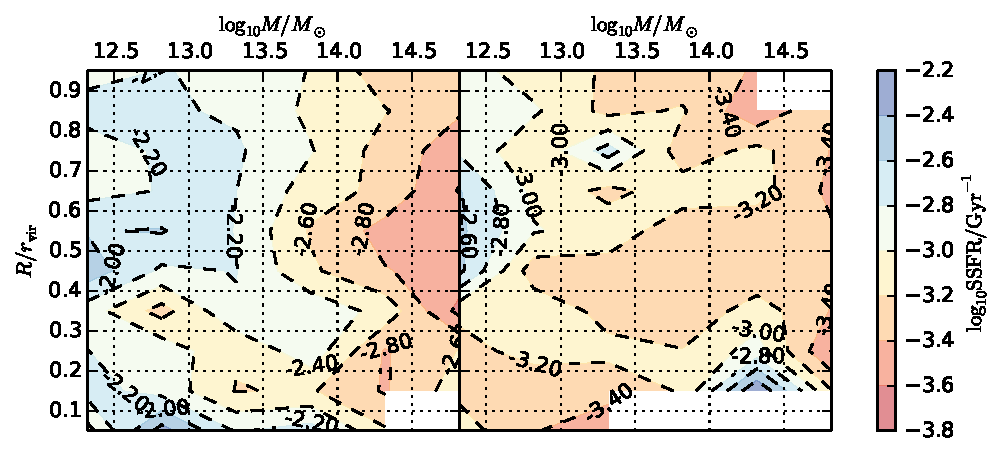
\includegraphics[height=0.2\textheight]{%
                    {figures/maggie_vs_sdss/tempel.0.mean_ssfr_2}.pdf%
                }
            }
        \end{minipage}
        \begin{minipage}{\linewidth}
            \centering
            \subfloat[Catalogue 5]{%
                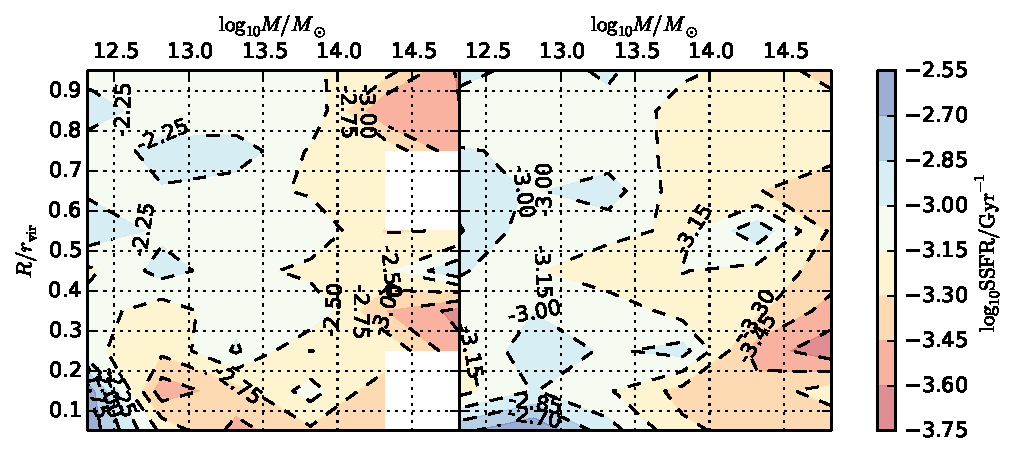
\includegraphics[height=0.2\textheight]{%
                    {figures/maggie_vs_sdss/tempel.0.mean_ssfr_4}.pdf%
                }
            }
        \end{minipage}
        \captionof{figure}{Same as \bartreffigure{ssfr_mean} but for galaxy
        groups from~\cite{Tempel+14}.\label{fig:ssfr_mean_tempel}}
    \end{minipage}
    \begin{minipage}{\linewidth}
        \centering
        \begin{minipage}{\linewidth}
            \centering
            \subfloat[Catalogue 3]{%
                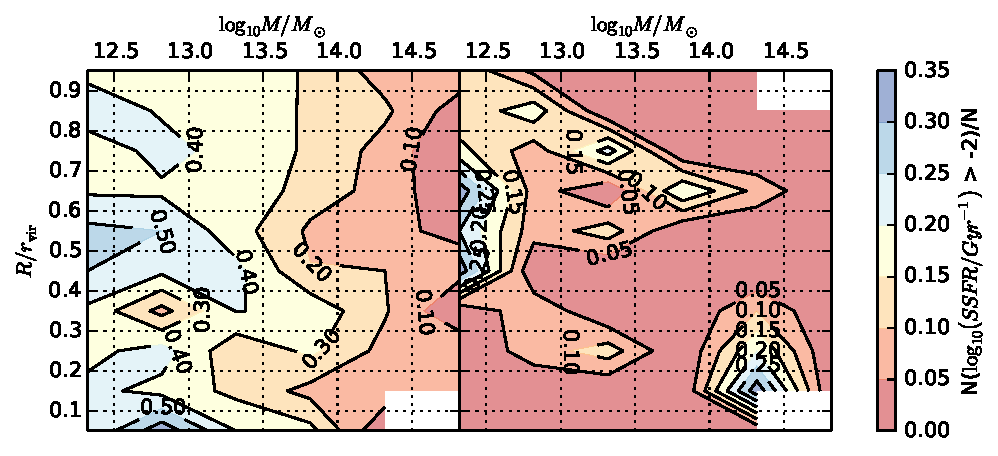
\includegraphics[height=0.2\textheight]{%
                    {figures/maggie_vs_sdss/tempel.0.fraction_over_minus_2_2}.pdf%
                }
            }
        \end{minipage}
        \begin{minipage}{\linewidth}
            \centering
            \subfloat[Catalogue 5]{%
                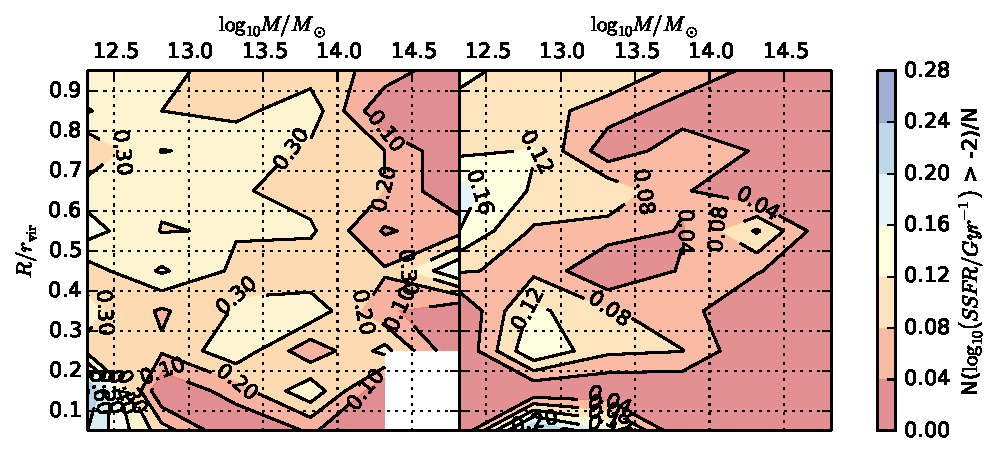
\includegraphics[height=0.2\textheight]{%
                    {figures/maggie_vs_sdss/tempel.0.fraction_over_minus_2_4}.pdf%
                }
            }
        \end{minipage}
        \captionof{figure}{Same as \bartreffigure{ssfr_fraction} but for
        galaxy groups
    from~\cite{Tempel+14}.\label{fig:ssfr_fraction_tempel}}
    \end{minipage}
\end{figure}
%
The modulation of the SSFR and fraction of young galaxies is very dependent of
the catalogue of groups used. Since these results between the two algorithms, a
deeper analysis must be done to understand from where the discrepancies come
from.

Still for MAGGIE, we plan to improve the galaxy grouping by the use of the
red-blue segregation of galaxies. We can use some priors for the modulation of
the fraction of blue galaxies in groups to adapt the probability computation
according to the class of the galaxy. Then, we can iteratively reduce the
impact of our initial model for the blue fraction by using the informations
obtained by MAGGIE to de-project the red-blue segregation observed in groups.
For next iterations, we can re-use our new real space model in the probability
computation, and do it until the convergence of memberships.

In parallel, we plan to launch a collaborative project with other grouping
algorithm developers. We will propose to each developer (and myself) to apply
their algorithms to a set of mock catalogs constructed in the same way to avoid
cosmic variance on the results, for blind tests. Then, we will run the same
tests on each algorithm in order to have a clear understanding of the strengths
and weaknesses of each of them. It will be the first time that galaxy grouping
algorithms will be compared in the same conditions.

Given that imperfect grouping algorithms wash out the observable environmental
effects, it is also interesting to know if there is a limit to recover the real
space modulation of galaxy properties (such as specific star formation rate)
with environment when trying to extract it from projected redshift space. This
can be easily done by imposing ourselves a modulation in the outputs of galaxy
formation codes, and then construct galaxy mock catalogues in redshift space.
We can then see if the imposed modulation is recovered in the observations, and
if galaxy group algorithms introduce biases in some cases. This will allow one
to determine the maximum level of environmental dependence of star formation
quenching that is consistent with the observations.

In continuation with the thesis work, we can try to theoretically explain the
observed dependency of galaxy properties with their environments. Using
hydrodynamical simulations of galaxies in groups, we wish to understand and
model intra-cluster physical processes (ram pressure stripping, tidal
stripping\ldots). This will imply running academic simulations independently
for each physical process, then model as a function of the different input
parameters (local and global environment essentially). And by trying to switch
them on-off in semi-analytical codes of galaxy formation, determine their
relative importance on galaxy properties (sSFR, bulge to disk ratios\ldots).

% vim: set tw=79 :
